%----------------------------------------------------------------
% FEUILLE DE STYLE ENSG au format Latex
% Création : sept. 2010 (D Lercier)
% Modification sept. 2012 (T Coupin)
%----------------------------------------------------------------

\documentclass{themeensg}

%---Texte en filigranne---
%pour l'enlever : \SetWatermarkText{}
%-------------------------

%---Mes packages à moi---
%\usepackage{}
%------------------------

%---Mes raccourcis---
\newcommand{\transpose}[1]{{}^t \! #1}
\newcommand{\ensg}{\textsc{Ensg}}
%--------------------

%---Paramètres du pdf---
    \hypersetup{
       backref=true,                           % Permet d'ajouter des liens dans
       pagebackref=true,                       % les bibliographies
       hyperindex=true,                        % Ajoute des liens dans les index.
       colorlinks=true,  %Colorise les liens : true pour version numérique, false pour version d'impression
       breaklinks=true,                        % Permet le retour à la ligne dans les liens trop longs.
       urlcolor= blue,                         % Couleur des hyperliens.
       linkcolor= blue,                       % Couleur des liens internes.
       bookmarks=true,                         % Créé des signets pour Acrobat.
       %bookmarksopen=true,                    % Si les signets Acrobat sont créés,
                                               % les afficher complètement.
       pdftitle={Thème ENSG},                 % Titre du document.
                                               % Informations apparaissant dans
       pdfauthor={Thibault Coupin},                      % dans les informations du document
       pdfsubject={Feuille de style ENSG}           % sous Acrobat.
    }

%-----------------------



%-------------------------------------------------------------

\setcounter{tocdepth}{1} %profondeur de la table des matières

\title{Feuille de style \LaTeX~de l'\ensg\\Documentation plus que rapide\\Version provisoire du \today~à \timenow}

%
%-------------------------------------------------------------
% Début du document
%--------------------------------------------------------------
\begin{document}
%--------------------------------------------------------------
\begin{titlepage}
%Inclusion des labels des entreprises
%Pour un seul label (à gauche), mettre NULL pour les 3e et 4e argument
\enterprise 
{logos/logo_ensg.jpg}
{Ecole Nationale des Sciences Géographiques}
{logos/logo_ensg.jpg}
{Ecole Nationale des Sciences Géographiques}

%Inclusion du titre
\maketitle{Stage de fin d'études \\Cycle des Ingénieurs diplômés de l'ENSG 3\up{ème} année }{logos/logo_ensg.jpg}

\infos{Mohamed-Amjad LASRI}{Septembre 2015}
\end{titlepage}


%---Page du jury---
%---Page du jury---
\newevenpage
\thispagestyle{plain}
\section*{Jury}
\vspace{0.5cm}

\textbf{Président de jury :} \\

Pierre-Yves Hardouin, directeur des enseignements de l'ENSG

\vspace{0.5cm}

\textbf{Commanditaire :} \\

KYLIA


Laboratoire d’Opto-Electronique, Métrologie et Instrumentation (LOEMI), Institut de l’Information Géographique et Forestière (IGN)

\vspace{0.5cm}

\textbf{Encadrement de stage :} \\ 

Olivier Martin IGN/DRE/SRSIG/LOEMI

Frédéric Verluise KYLIA

Emmanuel Bardière ENSG

\vspace{0.5cm}

\textbf{Responsable pédagogique du cycle Ingénieur :} \\

Serge Botton, IGN/ENSG/DE/DPTS

\vspace{0.5cm}

\textbf{Tuteur du stage pluridisciplinaire :} \\

Patricia Parisi, IGN/ENSG/DE/DSHI

\vspace{1cm}

\copyright \hspace{0.3cm} ENSG

\section*{Stage de fin d'étude du 04/05/2015 au 04/10/2015 }
\vspace{0.3cm}
\textbf{Diffusion web :} $\boxtimes$ Internet \hspace{0.2cm}$\boxtimes$ Intranet Polytechnicum\hspace{0.2cm}
$\boxtimes$ Intranet ENSG\vspace{0.3cm}

\textbf{Situation du document :} 
\vspace{0.2cm}
\par
Rapport de stage de fin d'études présenté en fin de 3\up{ème} année du cycle des Ingénieurs
\vspace{0.3cm}


\newcounter{x}
\setcounter{x}{\getpagerefnumber{LastPage}-\getpagerefnumber{beginappendices}+1}

\textbf{Nombres de pages :} 50 pages dont 3 d'annexes
\vspace{0.3cm}

\textbf{Système hôte :} \LaTeX
\vspace{1cm}


\textbf{Modifications :} 
\begin{center}
\begin{tabular}{|c|c|c|>{\centering}p{6.5cm}|}
\hline 
EDITION & REVISION & DATE & PAGES MODIFIEES\tabularnewline
\hline
\hline 
1 & 0 & 09/2015 & Création\tabularnewline
\hline 

\end{tabular}
\end{center}
%------------------

%------------------------------------------------------------------------------
% Remerciements
%\newevenpage
\chapter*{Remerciements}

Je tiens à remercier toutes les personnes qui ont participé de différentes façons à la réussite de mon stage et plus particulièrement les personnes que je cite ci-dessous.

Olivier MARTIN, Frederic VERLUISE, Christian THOM et Christophe MEYNARD qui m'ont encadré, conseillé et ont répondu régulièrement à mes questions tout au long de mon stage.

Emmanuel BARDIERE, mon référent de stage ENSG, qui a suivi l'évolution de mon stage tout au long de ces cinq mois.

Tout le personnel du Laboratoire d'Opto-Électronique et de la société KYLIA.



%---Résumé (français)---
\begin{abstract}
\thispagestyle{empty}
	\vspace{1cm}

	Ceci est mon résumé
	
	\vspace{1.5cm}
	
	\textbf{Mots clés :} clés, clés, clés
\end{abstract}
%-----------------------


%---Résumé (anglais)---
\selectlanguage{english}
\begin{abstract}
\thispagestyle{empty}
	\vspace{1cm}
	
	This is my abstract
	
	\vspace{1.5cm}
	
	\textbf{Key words:} key, key, key
\end{abstract}
%----------------------

\selectlanguage{frenchb}

%---Table des matières, des figures et des tableaux---
%\newevenpage
\tableofcontents

\newevenpage
\listoffigures

\newevenpage
\listoftables
%----------------------------------------------------

%\newevenpage
\chapter*{Glossaire et sigles utiles}
\addcontentsline{toc}{chapter}{Glossaire et sigles utiles}

  \begin{acronym}
  \acro{ENSG}{\'Ecole Nationale des Sciences Géographiques}
  \acro{GNSS}{Global Navigation Satellite Systems}
  \acro{GPS}{Global Positionning System}
  \end{acronym}


%---Introduction------------------------------------------------------------------
\newevenpage
\chapter*{Introduction}
  \addcontentsline{toc}{chapter}{Introduction}
  
  \vspace{1.5cm}
  
	La communication en champ proche (NFC) est une méthode de communication utilisée pour l'identification des personnes et des objets

%-------------------------------------------------------------------------------

\evenchapter[Concepts clés et problématiques]{Concepts clés et problématiques}

\textit{Le lecteur est prié de prêter une attention particulière au tableau des sigles lors de la lecture du présent document. Les protocoles qu'on présente utilisent un certain nombre d'abrévéations conventionnelles pour désigner Les opérations d'échanges entre. }

\section{Les Géocubes}
La miniaturisation des capteurs ainsi que la baisse des coûts de fabrication et de la consommation électrique des puces GNSS sont des facteurs qui peuvent laisser à envisager d'abandonner sur le terrain un réseau de capteurs opérant en permanence. Certains de ces capteurs GNSS permettent d'effectuer des mesures sur la phase donnant la possibilité de remonter à des précisions millimétriques, d'où l'idée d'un réseau de Géocubes. Le système Géocube est un réseau de capteurs GPS conçu et développé par le Laboratoire d'Opto-Éléctronique de Mesure et d'Instrumentation de l'Institut Géographique et Forestière Nationale. Il a comme objectif de mesurer les déformations avec une précision millimétrique. Ce réseau de capteurs a la particularité d'être très peu gourmand en énergie. On peut envisager de l'abandonner dans un milieu difficilement accessible sans qu'on ait à se soucier de son alimentation continue en électricité. En plus d'un module radio, un Géocube peut supporter plusieurs couches de capteurs lui permettant de collecter un certain nombre d'informations sur son environnement.

Dans les premières versions du Géocube initiés par LOEMI, Un opérateur humain peut communiquer directement avec un géocube en utilisant une de ces méthodes:

\begin{itemize}
\item Liaison série filaire, qui permet d'envoyer des commandes  à travers l'interface en lignes de commandes de G3OS.
\item Radio: Un protocol propriétaire particulier (DigiMesh\textcopyright) est utilisé pour communiquer avec un Géocube.
\end{itemize}

Dans la version industrielle du Géocube maintenue par la société Kylia, une attention particulière est prêtée à l'étanchéité du boîtier qui le contient et à la robustesse du produit final. Ce choix crucial se justifie principalement par le fait qu'un réseau de Géocube peut être destiné à la surveillance environnementale en temps de crise et doit, par conséquence, être résistant aux conditions extremes que peut présenter un tel contexte.

Un réseau de Géocubes communique à travers le protocol radio DigiMesh\textcopyright et l'utilise aussi pour centraliser les mesures acquises par les Géocubes vers un ordinateur, appelé coordinateur. Le coordinateur est le composant central du réseau, il encapsule toute la logique liée au traitement et au stockage des données. Il permet aussi à l'utilisateur de lancer des séries de calculs, récupérer les résultats ou de communiquer avec un Géocube en lançant des commandes qui seront transmises par radio. La Figure\ref{fig:geocube_network} résume ce schéma de fonctionnement.

\begin{figure}[h!]
\centering
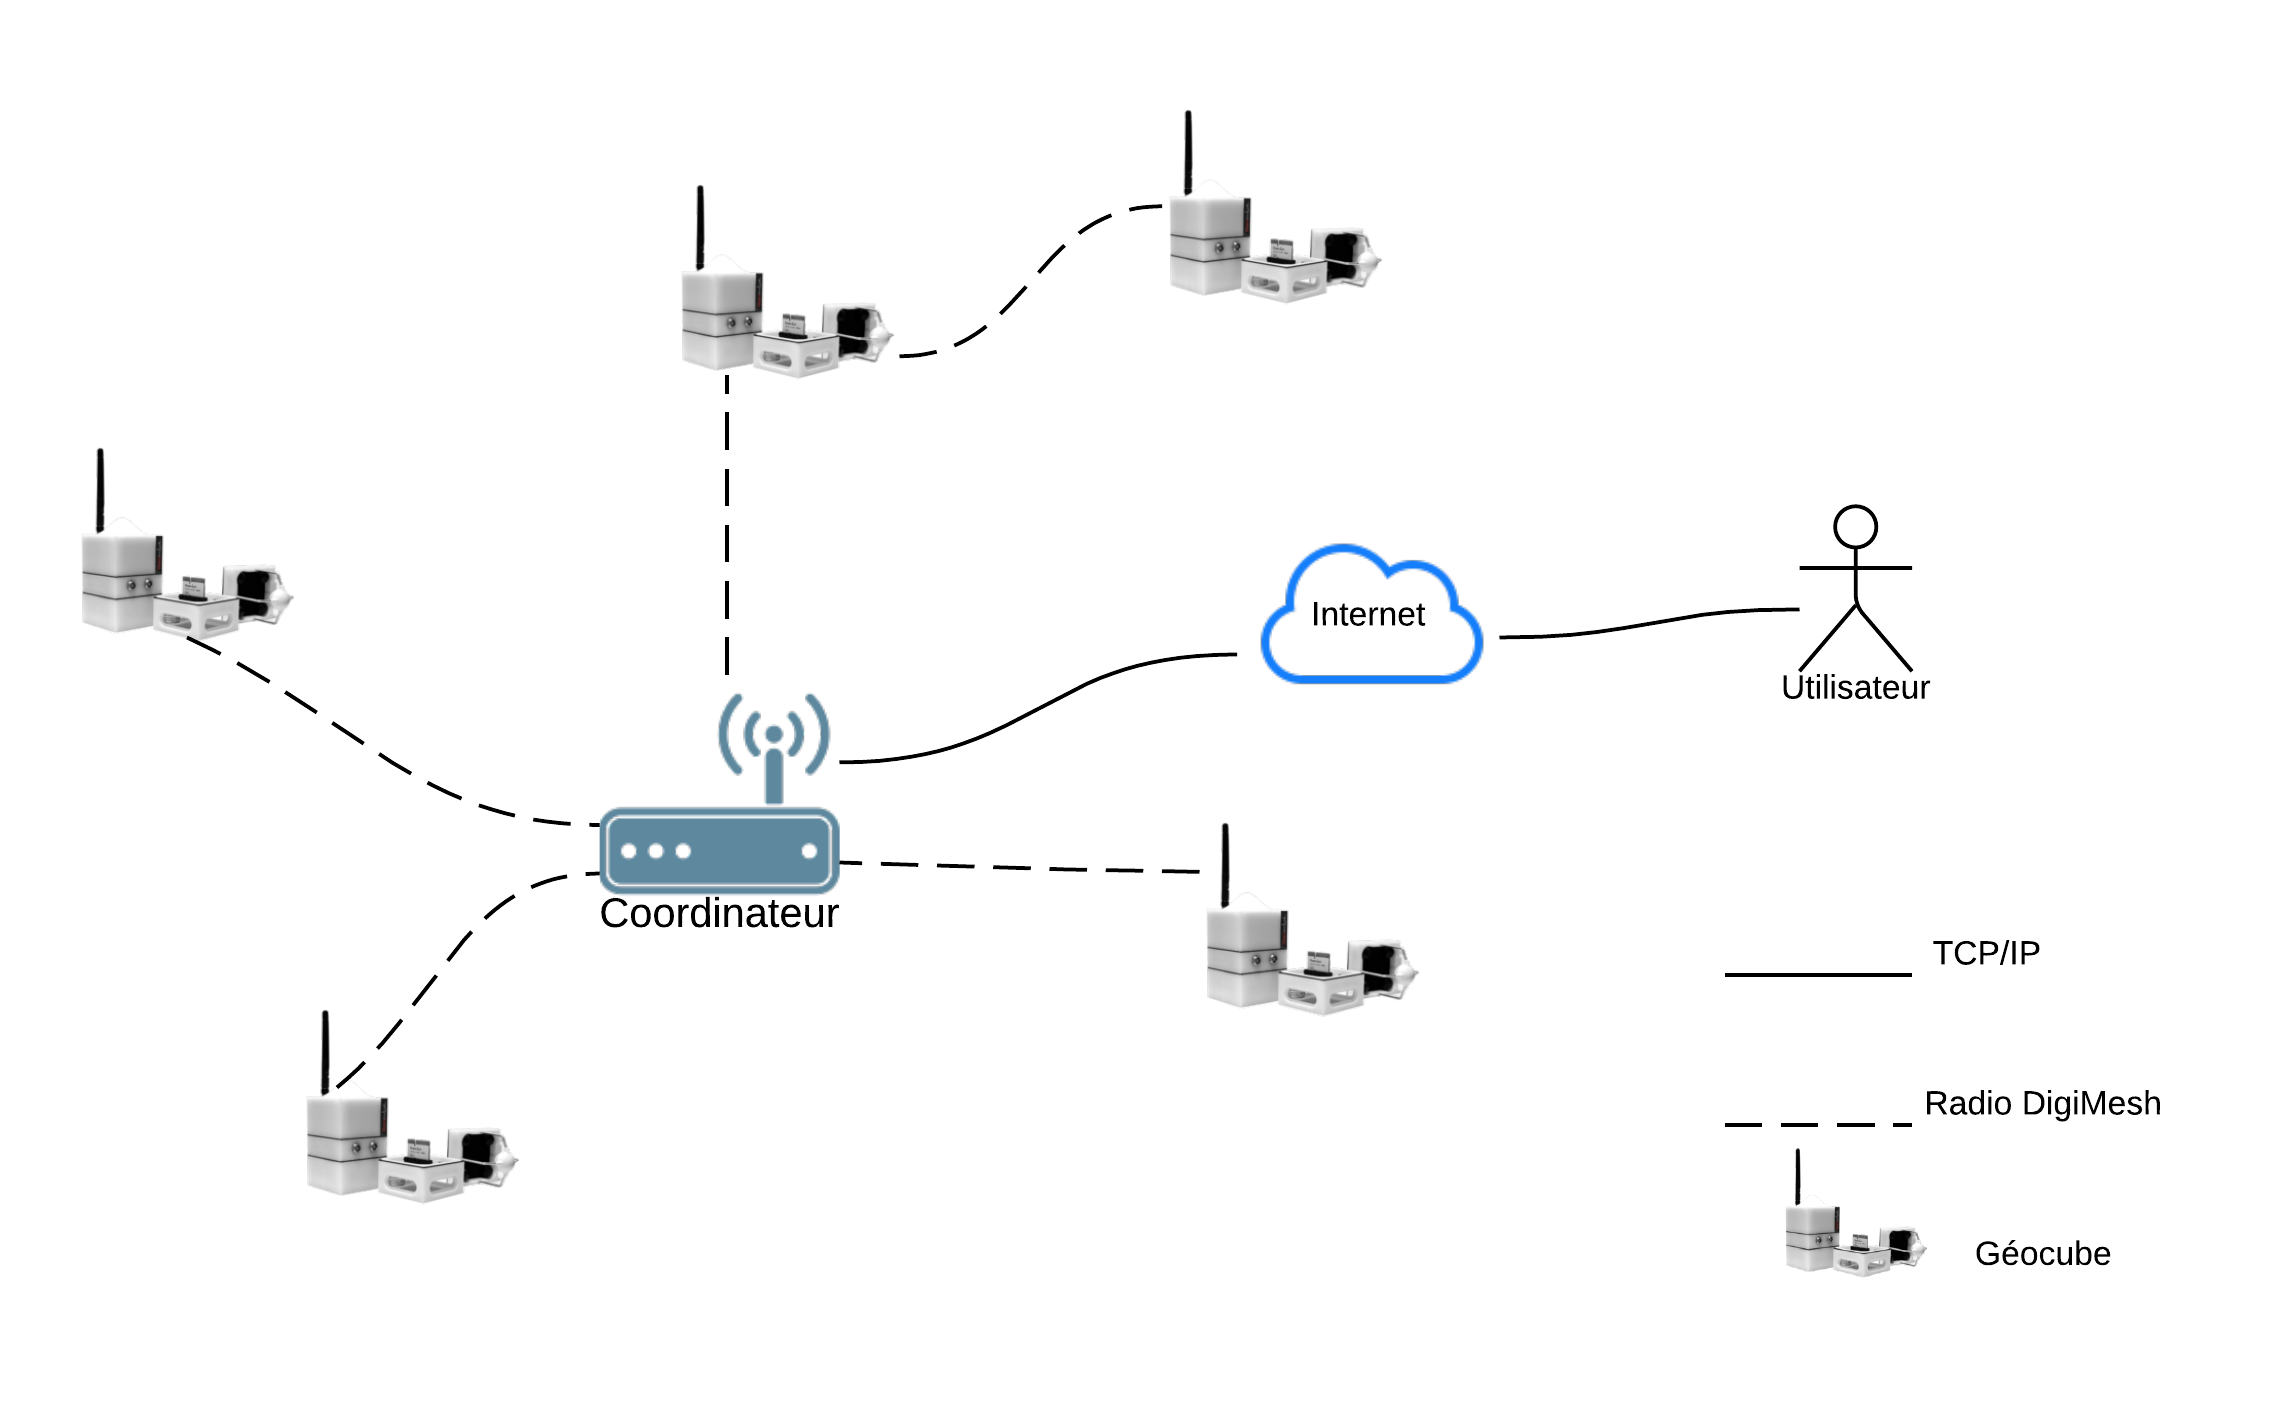
\includegraphics[scale=0.8]{images/fig1.png}
\caption{Un réseau de Géocubes}
\label{fig:geocube_network}
\end{figure}

\section{Les systèmes embarqués et les noyaux temps-réel dur:}


\begin{comment}
\begin{itemize}
\item \texttt{themeensg.cls} : contient les personnalisations et macros utiles
\item \texttt{jury.tex} : pour la feuille de présentation du jury
\item le dossier \texttt{images} : il doit contenir toutes les images, il contient déjà le dossier logo avec celui de l'\ensg
\item \texttt{bibliographie.bib} contient la bibliographie
\end{itemize}
\end{comment}
\section{Commandes personnalisées}

\begin{itemize}
\item \verb!\newevenpage! : identique à \verb!\newpage! mais en insère une page blanche de façon à débuter la nouvelle page sur un numéro de page impaire.
\item \verb!\evenchapter{titre}! : démarre un nouveau chapitre sur une page impaire,\\ \verb!\evenchapter[titre sommaire]{titre}! fonctionne aussi mais pas \verb!\evenchapter*{titre}!
\item idem pour \verb!\evenpart{titre}!
\end{itemize}

\section{Fichier source de cette doc}
Ce fichier \texttt{tex} contient toute la structure d'un rapport mais une bonne partie est désactivée car commentée par l'environnement \verb!\begin{comment} ... \end{comment}!


%-------------------------------------------------------------------------------
\newevenpage
\chapter*{Conclusion}
  \addcontentsline{toc}{part}{Conclusion}
  \vspace{1.5cm}
Il est l'heure de conclure : bonne nuit !


%-------------------------------------------------------------------------------
% Insertion de la bibliographie
\newevenpage
\nocite{*}
\bibliographystyle{apalike}
\bibliography{bibliographie}

\newevenpage
\begin{appendices} 
\label{beginappendices}
\annexe[Filtre de Kalman]{Filtre\newline de Kalman}
\label{annexekalman}
Annexe 1

\end{appendices} 

\end{document}